\chapter{Schnittstelle iCloud}
Patrick Niepel, Marcel Hagmann, Carl Philipp Knoblauch

\section{Einleitung}
In diesem Abschnitt wird die Schnittstelle mit iCloud beschrieben. Dabei wird erklärt wie die Architektur aufgebaut ist, wie mit der Schnittstelle kommuniziert wird und welche Probleme aufgetreten sind. 

\section{Warum iCloud/CloudKit?}

Wenn man bei der Entwicklung einer iOS App auf Cloud Services zurückgreifen will, bietet sich natürlich das Apple eigene CloudKit für iCloud an. Es ergab sich dadurch auch die Möglichkeit eine neues Framework kennenzulernen, da wir zuvor noch nicht mit CloudKit gearbeitet hatten. 
Über die Cloud-Schnittstelle sollen zwischen Lehrer und Schüler alle Aufgaben geteilt werden. Der Lehrer kann seine Aufgaben/Spiele in iCloud laden und diese mit seinen Schülern teilen. Die Schüler sollen dann diese Aufgaben/Spiele erledigen und ihre Lösungen wieder in iCloud laden. Dadurch wird dem Lehrer wiederum ermöglicht sich einen Überblick über die Lösungen seiner Klasse zu machen. Mit CloudKit konnten wir diese Ziele alle umsetzten.

\section{Architektur}


\begin{figure}
  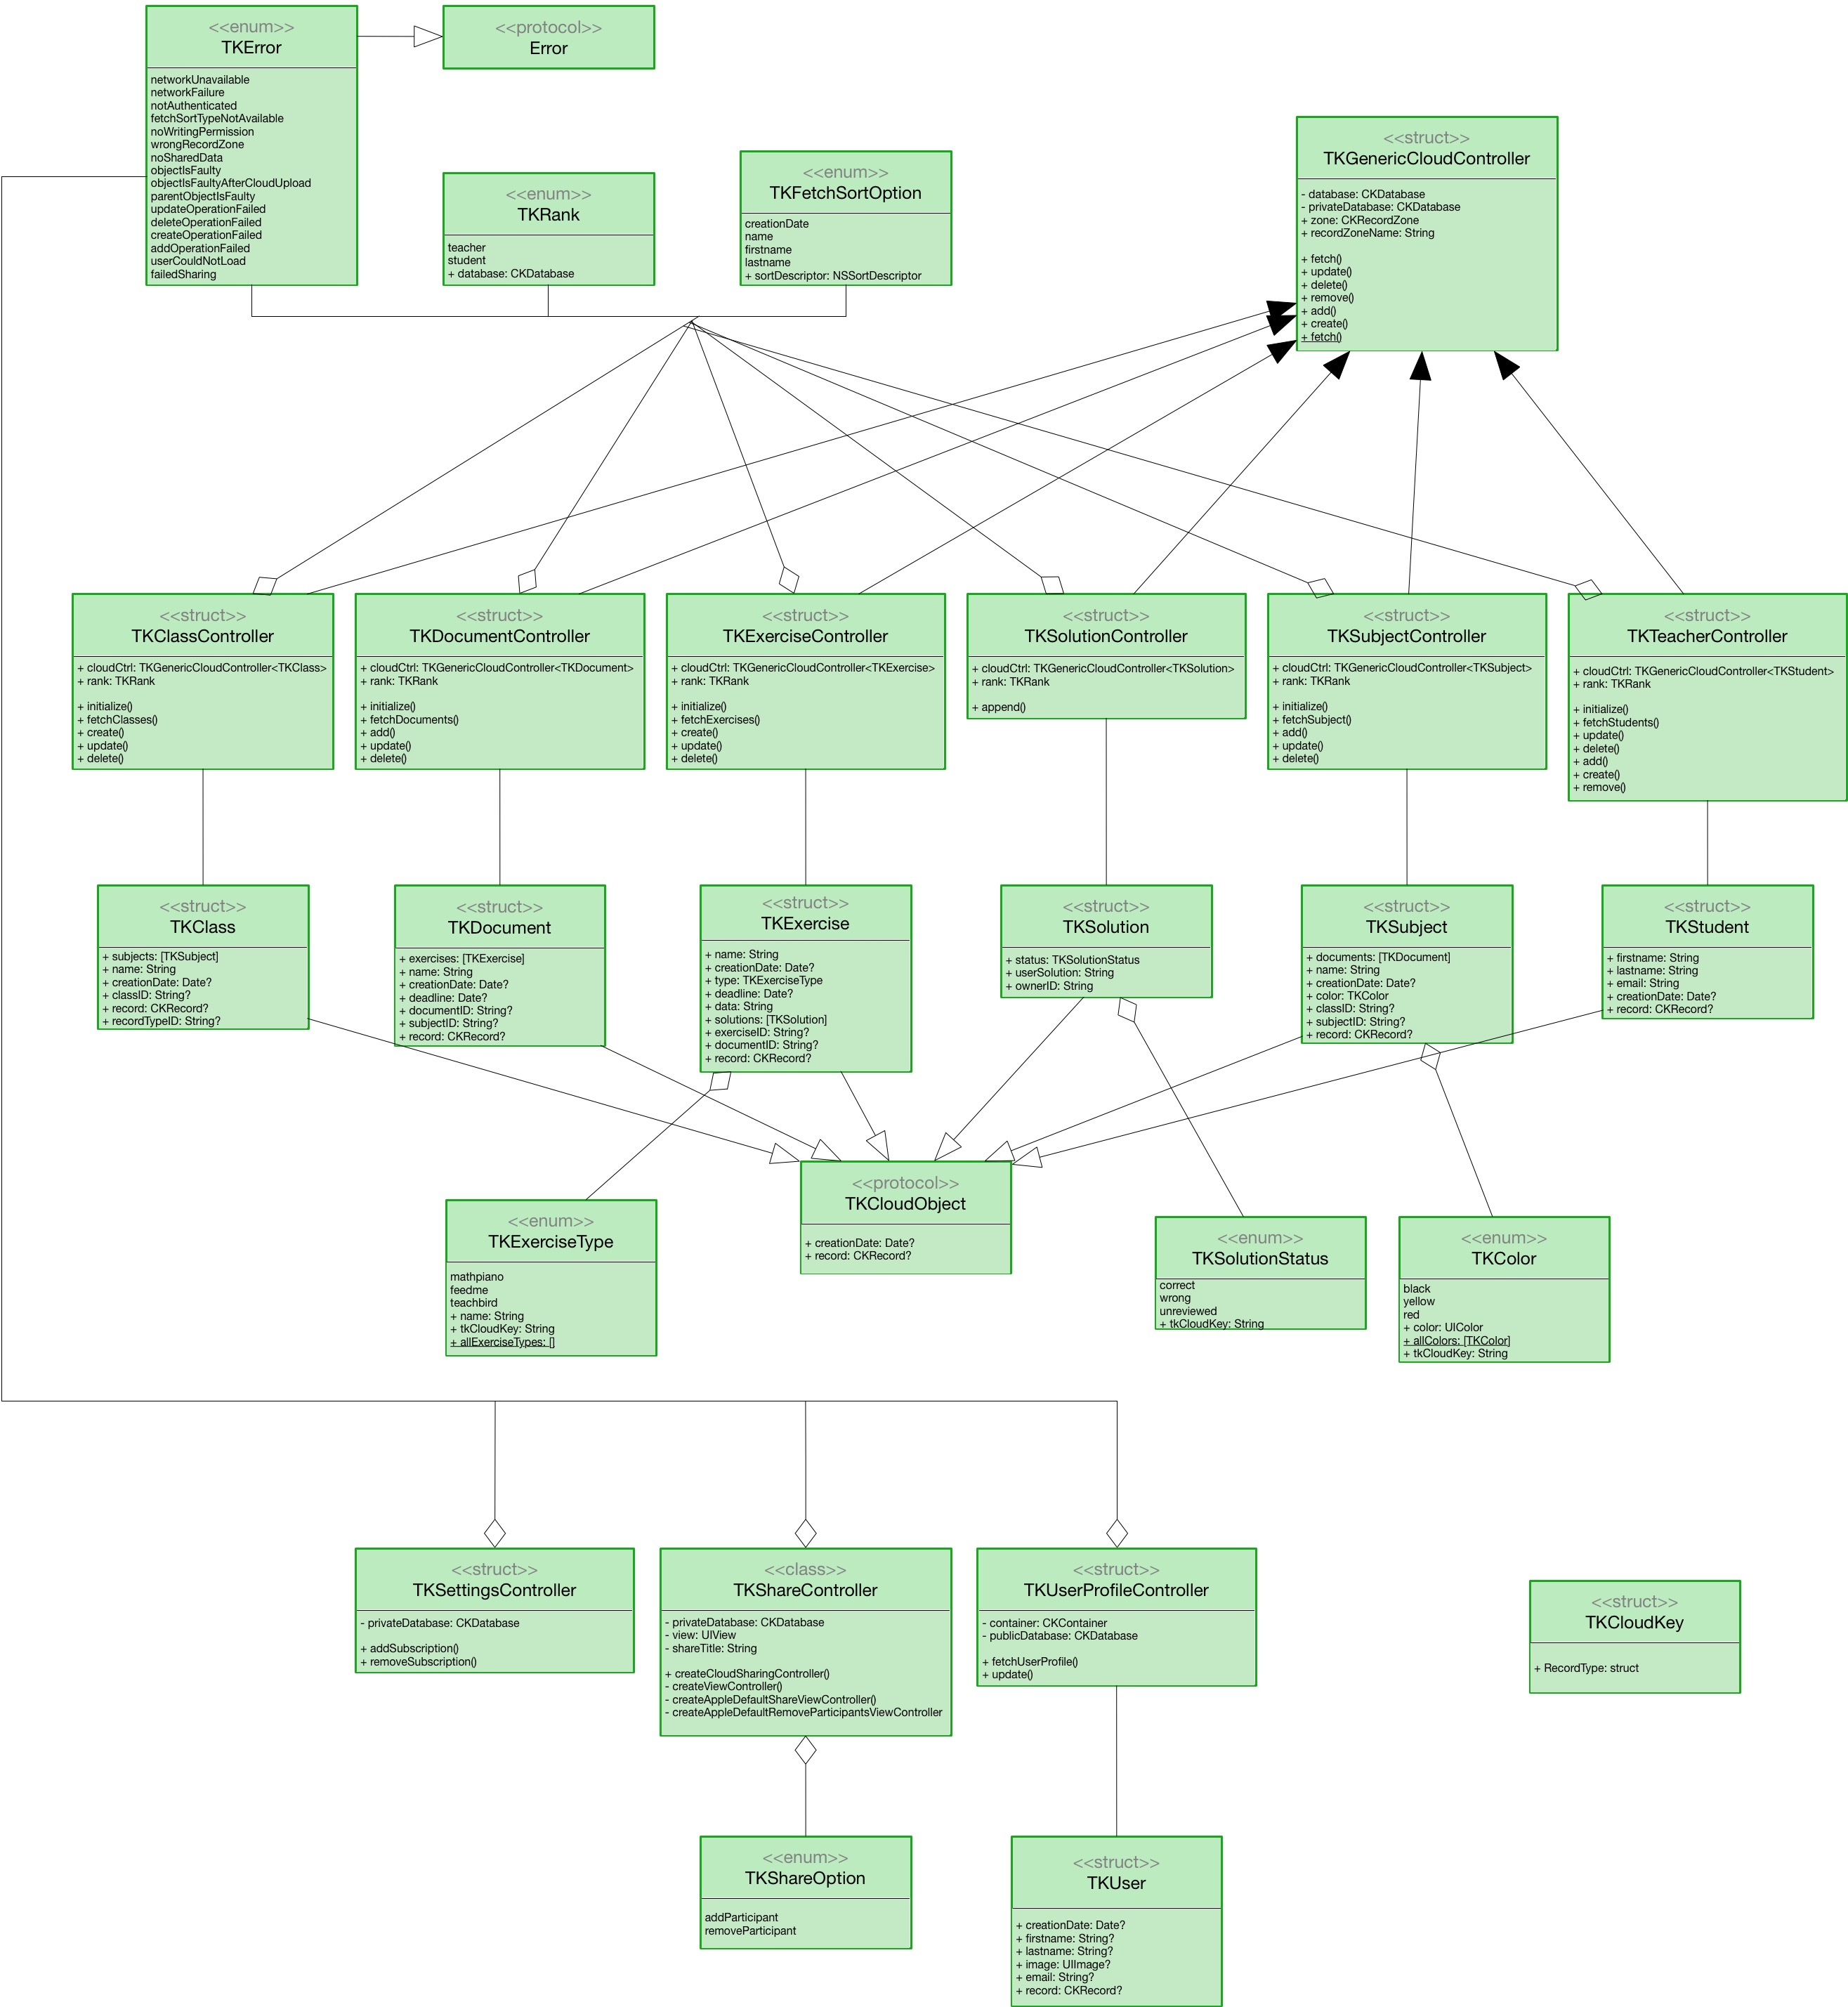
\includegraphics[width=\linewidth]{images/Klassendiagram_TeachKit.jpg}
  \caption{TeachKit Schnittstellen Klassendiagramm}
  \label{fig:boat1}
\end{figure}

Auch TeachKit ist strikt nach der Model-View-Controller - Architektur aufgebaut. Hierbei erben alle Models, die in der Cloud gespeichert werden, von ihrer Superklasse TKCloudObject. Die Controller die diese Models verwalten, sind mit Hilfe eines generischen Controllers TKGenericCloudController implementiert worden. Alle Cloud-Models und Controller bedienen sich von verschiedenen Enumerations, die die Funktionalität übersichtlicher gestalten.

\newpage


\section{Features}

\subsection{Upload/Download/Delete/Fetch/Update}

Für jeden Datentyp in TeachKit, gibt es einen Controller der für die Operationen auf den Datentyp verantwortlich ist.
Somit gibt es folgende Controller für die Datentypen:

\begin{itemize}

\item TKClassController
\item TKSubjectController
\item TKDocumentController
\item TKExerciseController
\item TKSolutionController

\end{itemize}

Alle Controller sind ähnlich aufgebaut. Der Grund weshalb der Controller über die Methode initialize(…) funktionsfähig gemacht werden muss ist der, dass der Student auf die Shared-Database zugreift und diese zuerst gefetched werden muss.

Um doppelten Code zu vermeiden, arbeiten alle der oben genannten Controller mit dem TKGenericCloudController, der die Grundfunktionen übernimmt und in den jeweiligen Controllern dann spezialisiert werden.

\subsection{User Profile}

Zu jedem Nutzer kann der Vorname, Nachname und ein Profilbild gespeichert werden. Der TKUserProfileController der für die Nutzerverwaltung verantwortlich ist, arbeitet auf der Public-Database. Das bedeutet, dass alle Nutzer diese Informationen sehen können. Die aktuelle implementation erlaubt nur den download der Daten für den derzeit eingeloggten Nutzer. Diese kann erweitert werden, hätte aber momentan keine Verwendung gefunden.

\subsection{Sharing}

Eines der wichtigsten Features unserer App ist das Teilen von Daten zwischen Teacher und Student. Nach dem Teilen gemeinsamer Daten haben beide Zugriff auf das Subject und alles was darunter angelegt ist.

CloudKit arbeitet mit drei verschiedenen Datenbanken.



\subsection{Push/Subscriptions}


\subsection{TKError}

\section{Aufgetretene Probleme}

\subsection{Subscription}

\subsection{Sharing}

\subsection{TKSolution}